\documentclass[11pt]{beamer}
\usetheme{CambridgeUS}
%\usepackage[utf8]{inputenc}
%\usepackage[turkish]{babel}
\usepackage{amsmath}
\usepackage{amsfonts}
\usepackage{amssymb}
\usepackage{graphicx}
\usepackage{listings}

\definecolor{lbcolor}{rgb}{0.95,0.95,0.95}  
\lstset{  
	language=Python,  
	tabsize=4,  
	basicstyle=\ttfamily,  
	backgroundcolor=\color{lbcolor},  
	showstringspaces=false,
	frame=single,
	frameround=tttt
}


\author{Prof.Dr.Mehmet Hakan Satman \\ mhsatman@istanbul.edu.tr}
\title{Scientific Computing and (Big) Data Analysis with Julia}
\setbeamercovered{transparent} 
%\setbeamertemplate{navigation symbols}{} 
\logo{
\includegraphics[width=1cm]{images/iulogo.jpg}} 
\institute{Istanbul University} 
\date{2023.12.01} 

\begin{document}

\begin{frame}

\includegraphics[width=1cm]{images/julia.png}
\titlepage
\end{frame}

\begin{frame}[fragile]{Julia Programming Language}{julialang.org}
	\begin{center}
		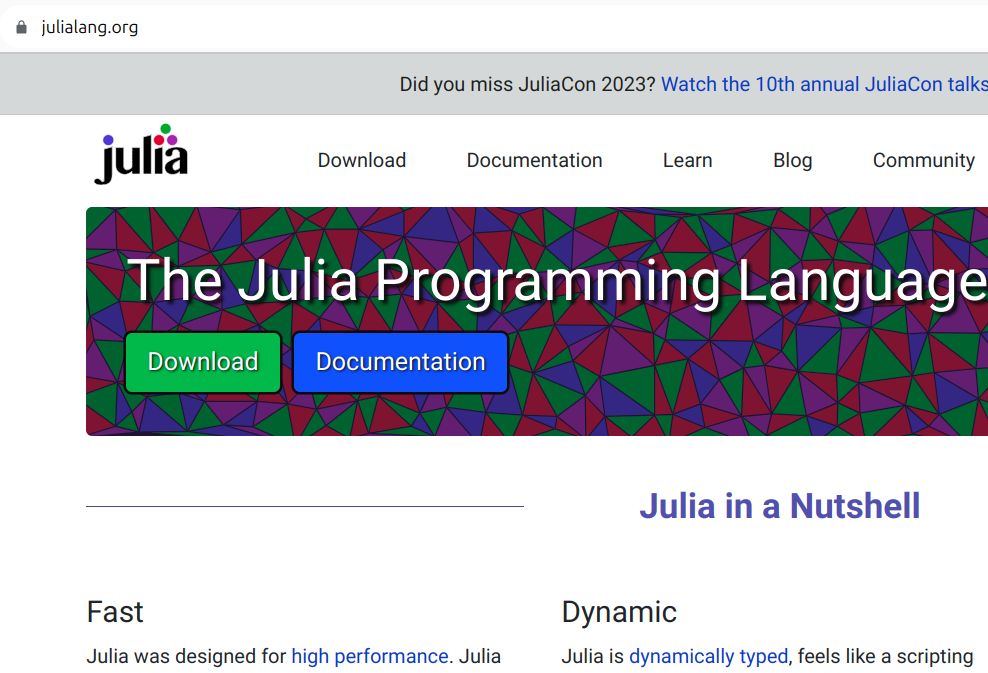
\includegraphics[width=8cm]{images/thesite.png}
	\end{center}
\end{frame}


\begin{frame}[fragile]{Julia Programming Language}{High Performance Computing}
\begin{itemize}
	\item Julia was designed for high performance. Julia programs automatically compile to efficient native code via LLVM, and support multiple platforms (Windows, MacOS, Linux, etc.)\footnote{\url{https://julialang.org/}}.
\end{itemize}
\end{frame}


\begin{frame}[fragile]{Julia Programming Language}{Dynamic}
	\begin{itemize}
		\item Julia is dynamically typed, feels like a scripting language, and has good support for interactive use, but can also optionally be separately compiled\footnote{\url{https://julialang.org/}}.
	\end{itemize}
\end{frame}


\begin{frame}[fragile]{Julia Programming Language}{Composable}
	\begin{itemize}
		\item Julia uses multiple dispatch as a paradigm, making it easy to express many object-oriented and functional programming patterns. The talk on the Unreasonable Effectiveness of Multiple Dispatch explains why it works so well\footnote{\url{https://julialang.org/}}.
	\end{itemize}
\end{frame}

\begin{frame}[fragile]{Julia Programming Language}{Open Source}
	\begin{itemize}
		\item Julia is an open source project with over 1,000 contributors. It is made available under the MIT license. The source code is available on GitHub\footnote{\url{https://julialang.org/}}.
	\end{itemize}
\end{frame}


\begin{frame}[fragile]{Julia Programming Language}{First things first!}
\begin{lstlisting}
println("Hello, world")
\end{lstlisting}
\end{frame}


\begin{frame}[fragile]{Julia Programming Language}{Welcome!}
	\begin{center}
			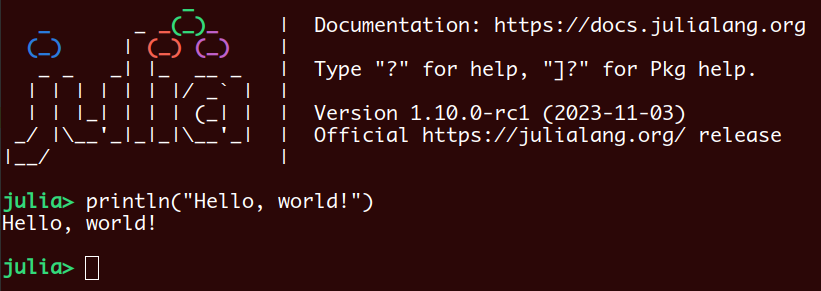
\includegraphics[width=10cm]{images/welcome.png}
	\end{center}
\end{frame}


\begin{frame}[fragile]{Julia Programming Language}{The editor: Visual Studio Code}
	\begin{center}
		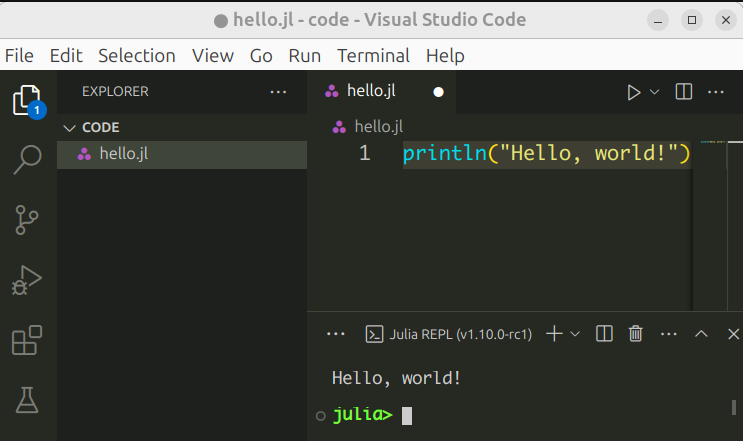
\includegraphics[width=10cm]{images/vscode.png}
	\end{center}
\end{frame}


\begin{frame}[fragile]{Linear Regression}{The formulation}
\begin{equation}
y = \beta_0 + \beta_1 x + \varepsilon
\end{equation}

\begin{equation}
	\hat{y} = \hat{\beta}_0 + \hat{\beta}_1 x 
\end{equation}

\begin{equation}
	\hat{\boldsymbol{\beta}} = (X'X)^{-1}X'y
\end{equation}
\end{frame}


\begin{frame}[fragile]{Linear Regression}{Sample Data}
\begin{equation}
X = \begin{bmatrix}
	1 & 1 \\
	1 & 2 \\
	1 & 3 \\
	1 & 4 \\
	1 & 5 
\end{bmatrix}, y = \begin{bmatrix}
2 \\
5 \\ 
5 \\ 
8 \\ 
12
\end{bmatrix}
\end{equation}
\end{frame}


\begin{frame}[fragile]{Linear Regression}{The Matrix Solution}
\begin{lstlisting}
using LinearAlgebra
		
x = [1, 2, 3, 4, 5]
y = [2, 5, 5, 8, 12]
X = hcat(ones(5), x)
betahats = inv(X'X)X'y
println(betahats)
\end{lstlisting}
	
\begin{lstlisting}
julia> include("reg-matrix.jl")
[-0.5, 2.3]
\end{lstlisting}
\end{frame}


\begin{frame}[fragile]{Linear Regression}{Pseudo Inverse - Numerical Fit}
\begin{lstlisting}
x = [1, 2, 3, 4, 5]
y = [2, 5, 5, 8, 12]

betahats = hcat(ones(5), x) \ y 
println(betahats)	
\end{lstlisting}

\begin{lstlisting}
julia> include("reg-simple.jl")
[-0.5, 2.3]
\end{lstlisting}
\end{frame}


\begin{frame}[fragile]{Linear Regression}{The GLM package}
\begin{lstlisting}
using GLM 

x = [1, 2, 3, 4, 5]
y = [2, 5, 5, 8, 12]

result = lm(hcat(ones(5), x), y)

println(result)

\end{lstlisting}
\end{frame}


\begin{frame}[fragile]{Linear Regression}{The GLM package - Results}
\begin{lstlisting}[basicstyle=\tiny]
julia> include("reg-glm.jl")
	
Coefficients:
------------------------------
	  Coef.  Std. Error   t     Pr(>|t|)  Lower 95%  Upper 95%
------------------------------
x1   -0.5    1.25565   -0.40    0.7171   -4.49605    3.49605
x2    2.3    0.378594   6.08    0.0090    1.09515    3.50485
------------------------------
\end{lstlisting}

\begin{lstlisting}
julia> GLM.r2(result)
0.9248251748251748
\end{lstlisting}


\end{frame}


\begin{frame}[fragile]{XOR}{eXclusive OR}
\begin{table}
\centering
\begin{tabular}{|c|c|c|}
	\hline
	$x_1$ & $x_2$ & $y$ \\
	\hline 
	1 & 1 & 0 \\
	\hline 
	1 & 0 & 1 \\
	\hline 
	0 & 1 & 1 \\
	\hline 
	0 & 0 & 0 \\
	\hline 
\end{tabular}
\caption{$y = \text{xor}(x_1, x_2)$}
\end{table}
\end{frame}

\begin{frame}[fragile]{Symbolic Regression}
\begin{lstlisting}
using SymbolicRegression, MLJ

x = (
	x1 = Float64[1, 1, 0, 0], 
	x2 = Float64[1, 0, 1, 0]
)
		
y = Float64[0, 1, 1, 0]
		
\end{lstlisting}
\end{frame}


\begin{frame}[fragile]{Symbolic Regression}
	\begin{lstlisting}
model = SRRegressor(
	niterations = 50,
	binary_operators = [+, -, *],
	unary_operators = [abs],
	should_simplify = true,
	save_to_file = false)

\end{lstlisting}
\end{frame}

\begin{frame}[fragile]{Symbolic Regression}
\begin{lstlisting}
mach = machine(model, x, y)
fit!(mach)
report(mach)
@info predict(mach, x)
\end{lstlisting}
\end{frame}


\begin{frame}[fragile]{Symbolic Regression}
\begin{lstlisting}
Hall of Fame:   
------------------                                                                                                                                    Complexity  Loss       Score     Equation                                                                                                                1           2.500e-01  3.604e+01  y = 0.5                                                                                                                4           0.000e+00  1.201e+01  y = abs(x1 - x2)
--------------------                                                                                                       
[ Info: [0.0, 1.0, 1.0, 0.0]

\end{lstlisting}
\end{frame}



\begin{frame}[fragile]{Clustering Multivariate Data}{kmedoids}
	\begin{center}
		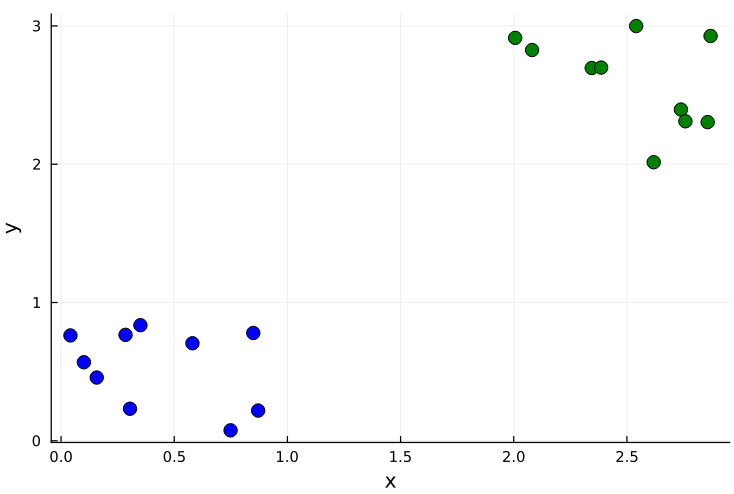
\includegraphics[width=8cm]{images/kmedoids1.png}
	\end{center}
\end{frame}

\begin{frame}[fragile]{Clustering Multivariate Data}{kmedoids}
	\begin{center}
		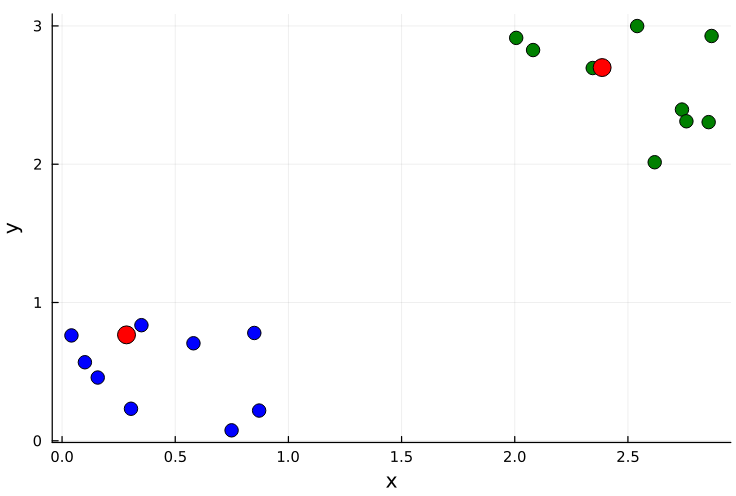
\includegraphics[width=8cm]{images/kmedoids2.png}
	\end{center}
\end{frame}

\begin{frame}[fragile]{Clustering Multivariate Data}{Problem of Distance Matrices}
\begin{lstlisting}
using Clustering, Plots, Distances

# data = Code for loading data...
plt = scatter(data[:, 1], data[:, 2])

dist = pairwise(euclidean, eachrow(data))

result = kmedoids(dist, 2)
centers = data[result.medoids, :];
scatter!(centers[:, 1], centers[:, 2])
\end{lstlisting}
\end{frame}


\begin{frame}[fragile]{Clustering Multivariate Data}{Problem of Distance Matrices}
\begin{lstlisting}
dist = pairwise(euclidean, eachrow(data))
\end{lstlisting}
\begin{itemize}
	\item A distance matrix holds the distance data of $ith$ and $jth$ points, e.g., $D(i, j) = D(j, i)$ due to the symmetry.
	\item If data has $n$ rows then the distance matrix is in dimension of $n \times n$. 
	\item Each distance is measured in 64-bits float numbers (\texttt{Float64}).
	\item If $n$ is large, your machine will probably throw an \emph{Out of Memory} error!
\end{itemize}
\end{frame}


\end{document}